\documentclass[12pt, letterpaper]{article}
\usepackage{graphicx}
\usepackage{graphicx}
\usepackage{polski}
\title{Generowanie danych}
\author{Anna Zadka, Natalia Klepacka, Kinga Teklak}

\begin{document}
	
\maketitle
	
\tableofcontents{}

\cleardoublepage

\subsection{klienci}
\subsubsection{Imię i nazwisko}
Imiona i nazwiska zostały pobrane ze strony \textbf{gov}, oddzielnie dla kobiet i mężczyzn. Następnie połączyłyśmy imiona damskie z nazwiskami oraz imiona i nazwiska męskie. Na koniec dane dla kobiet i mężczyzn zostały przemieszane. 
\textbf{https://dane.gov.pl/pl/dataset/1667,lista-imion-wystepujacych-w-rejestrze-pesel-osoby-zyjace}

\subsubsection{e-mail}

E-maile tworzyłyśmy z imion i nazwisk, oddzielonych kropką. Adres poczty zależy od podzielności indeksu nazwiska. W celu zachowania realizmu najczęstszym adresem poczty elektronicznej jest $@gmail.com$.

\begin{figure}[h!]
	\centering
	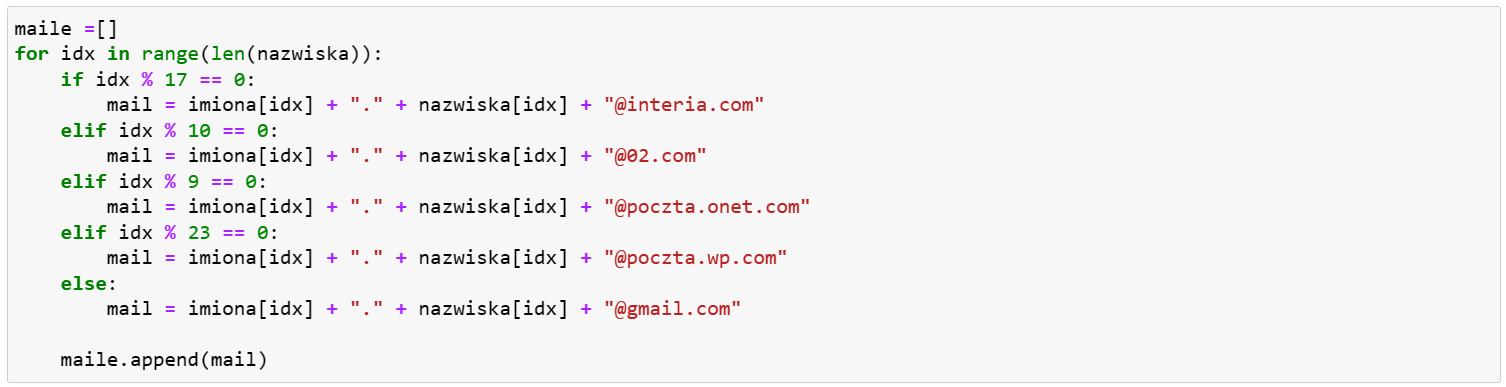
\includegraphics[width=1.0\textwidth]{1.png}
	\caption{Tworzenie e-maili.}
\end{figure}
\subsubsection{numer telefonu}
Numery telofonu są tworzone przez losowanie liczby pomiędzy $555555555$ a $777777777$ dla każdej osoby.
\begin{figure}[h!]
	\centering
	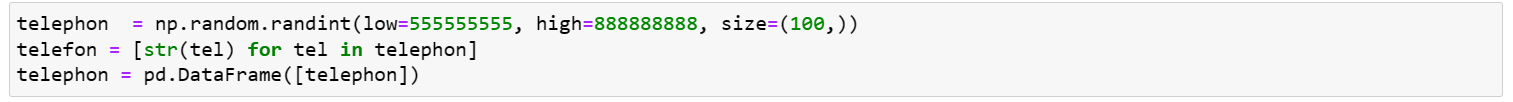
\includegraphics[width=1.0\textwidth]{2.png}
	\caption{Tworzenie numerów telefonu.}
\end{figure}




\subsection{gry}

\subsubsection{nazwa, gatunek, opis, minimalny wiek i możliwa liczba graczy}

Te informacje zostały skopiowane ze strony:
\textbf{https://www.gracula.pl/wypozyczalnia-listagier}.

\subsubsection{wydawnictwo}
Wydawnictwo zostało wylosowane ze zwracaniem z podanych:
\textit{"Nasza Księgarnia","Aleksander","Trefl","Muduko","Panini","Zielona Sowa","Rebel","Albi","Fishbone Games"}.

\subsubsection{cena wypożyczenia i kupna}
Ceny zostały stworzone poprzez wylosowanie liczby do $10$, w przypadku wypożyczeń i do $30$ w przypadku kupna. Następnie dodano do nich $0.99$.
\begin{figure}[h!]
	\centering
	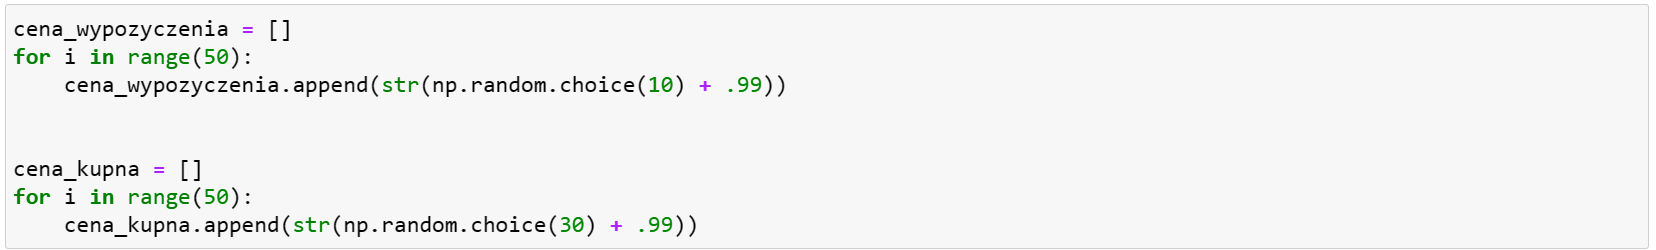
\includegraphics[width=1.0\textwidth]{3.png}
	\caption{Tworzenie cen wypożyczeń i kupna gier.}
\end{figure}


\subsection{pracownicy}
\subsubsection{imię, nazwisko, płeć, numer telefonu}
Od początku działania sklepu zostało zatrudnionych dziesięciu pracowników. Ich imiona, nazwiska i płeć zostały wylosowone jak wyżej za pomocą danych z \textbf{gov}. Numery telefonu zostały wylosowane jak powyżej.
\subsubsection{data urodzenia}
Data urodzenia pracowników jest wybierana jako data między rokiem $1970$, a $1990$.
\begin{figure}[h!]
	\centering
	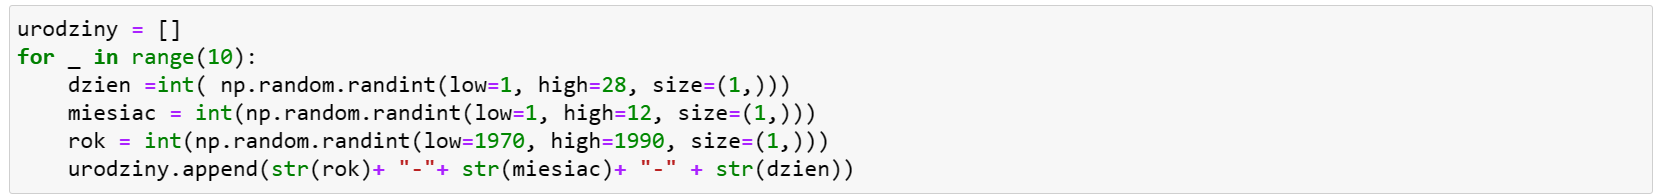
\includegraphics[width=1.0\textwidth]{4.png}
	\caption{Tworzenie daty urodzeń pracowników.}
\end{figure}

\subsubsection{adres}

Adresy składają się z wylosowanej ulicy we Wrocławiu lub jego okolicy(Kamień, Kiełczówek, Krzyżanowice, Łany), numeru domu od 1 do 120, miejscowości i kodu pocztowego.
\begin{figure}[h!]
	\centering
	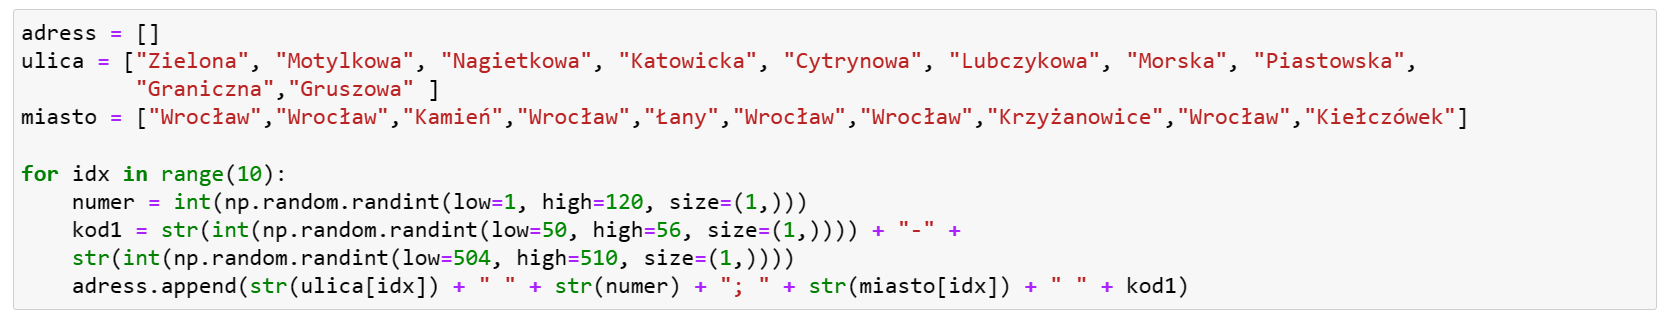
\includegraphics[width=1.0\textwidth]{5.png}
	\caption{Tworzenie adresów pracowników.}
\end{figure}

\subsubsection{data zatrudnienia}
Datę zatrudnienia pracowników tworzymy wybierając losową datę między rokiem 2013, a 2020. 
\begin{figure}[h!]
	\centering
	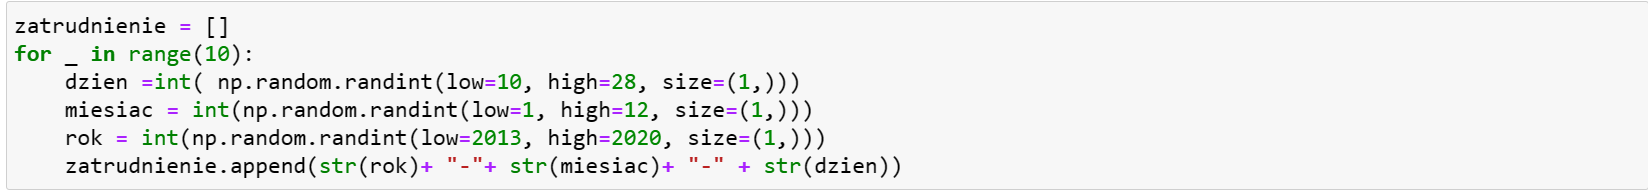
\includegraphics[width=1.0\textwidth]{6.png}
	\caption{Tworzenie daty zatrudnienia.}
\end{figure}


\subsection{pensje}
\subsubsection{pensja}
Pensje losujemy dla każdego pracownika(w przypadku zmiany kwoty pensji kolejny raz), wybierając kwote spośród następujących: $6653,3500,4400,4530,3550$.




\subsection{sprzedaże}

Losujemy liczbę sprzedaży z rozkładu Poissona z powiększającą się zmienną $\lambda$ (zaczynamy od 10 i zwiększamy o 0.001) dla każdego dnia działania sklepu. Następnie losujemy czas sprzedaży (czyli godzinę między 10 a 17 i minuty między 0 i 59), ponieważ założyłyśmy czas działania wypożyczalni od 10 do 18. Na koniec losujemy tytuł kupionej gry, który został sprzedany(używamy tutaj \textbf{random.choice}, ponieważ losujemy ze zwracaniem).
\begin{figure}[h!]
	\centering
	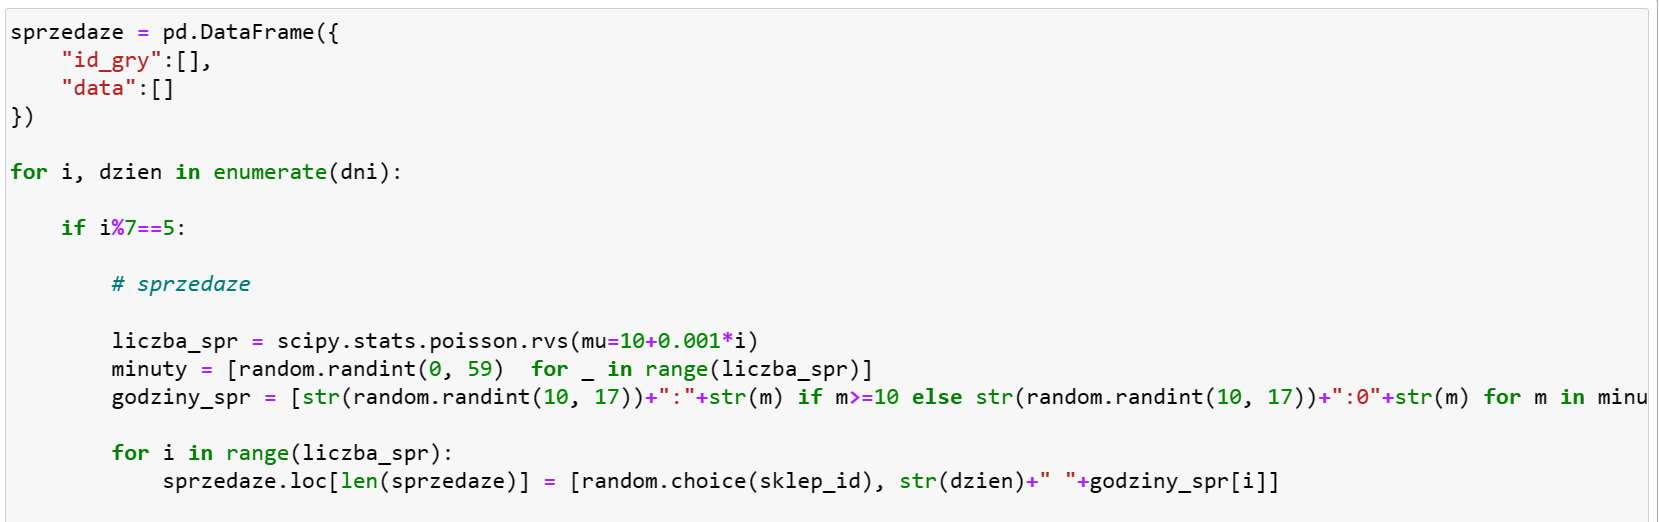
\includegraphics[width=1.0\textwidth]{8.png}
	\caption{Tworzenie sprzedaży dla każdego dnia.}
\end{figure}



\subsection{turnieje, wyniki}
Sposób generowania omówimy na przypadku dla roku 2023. Klasyfikacje odbyły się w kwietniu, finał natomiast się jeszcze nie odbył(dlatego w bazie nie ma id finału i wyników turnieju). Losujemy zawodników z listy zawodników i ich liczb, która jest maksymalną liczbą jaką dopuszcza gra do kwadratu. Robimy to, ponieważ w klasyfikacjach bierze udział więcej drużyn, a każdy kto wygra w swojej drużynie kwalifikuje się do finału. Jeśli zawodnik przechodzi do finału do punktów w tabeli wyniki wpisujemy 1, w przeciwnym wypadku 0.
W finale za pierwsze miejsce zawodnik dostaje 2 punkty, za ostatnie 0, a każdy kto nie zajął pierwszego lub ostatniego miejsca otrzymuje 1 punkt.
\begin{figure}[h!]
	\centering
	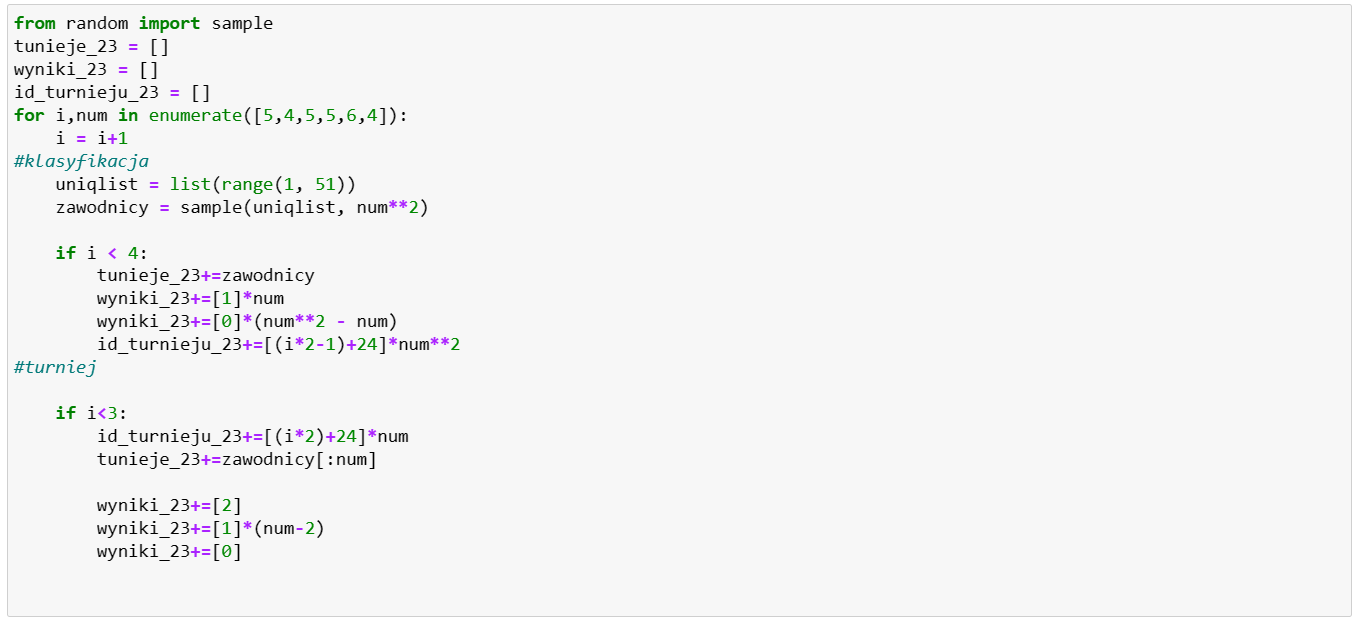
\includegraphics[width=1.0\textwidth]{9.png}
	\caption{Tworzenie tabeli turnieje i wyniki.}
\end{figure}




\subsection{wypożyczenia}

Dla każdego dnia tygodnia roboczego losujemy liczbę wypożyczeń z rozkładu Poissona z rosnącym parametrem $\lambda$(zaczynając od 2 i zwiększając o 0.001). Jeśli liczba wypożyczeń jest większa niż 0, to losujemy tytuł z dostępnych gier(używamy tutaj \textbf{random.sample}, ponieważ losujemy bez zwracania). Następnie wybieramy czas jej wypożyczenia (czyli godzinę między 10 a 17 i minuty między 0 i 59), ponieważ założyłyśmy czas działania wypożyczalni od 10 do 18.
Data zwrotu to liczba z rozkłądu Poissona z $\lambda = 2$ i średnią równą 3. Dla każdego zwrotu również losujemy czas analogicznie jak dla wypożyczeń. 
\begin{figure}[h!]
	\centering
	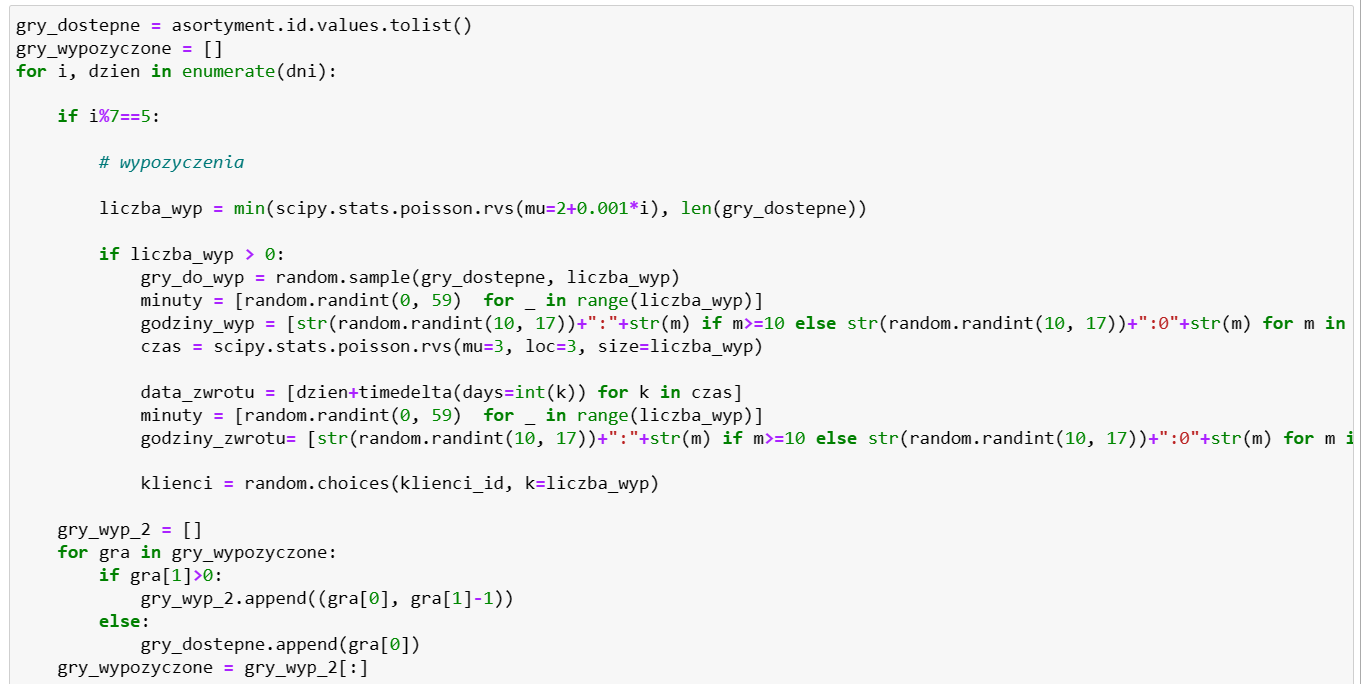
\includegraphics[width=1.0\textwidth]{7.png}
	\caption{Tworzenie wypożyczeń dla kazdego dnia działania sklepu.}
\end{figure}



	
\end{document}